% CS631 Advanced Programming in the UNIX Environment
% Author: Jan Schaumann <jschauma@netmeister.org>
% $Id: slides.tex,v 1.1 2005/11/20 18:42:12 jschauma Exp $

\documentclass[xga]{xdvislides}
\usepackage[landscape]{geometry}
\usepackage{graphics}
\usepackage{graphicx}
\usepackage{colordvi}
\usepackage[normalem]{ulem}

\begin{document}
\setfontphv

%%% Headers and footers
\lhead{\slidetitle}
\chead{CS631 - Advanced Programming in the UNIX Environment}
\rhead{Slide \thepage}
\lfoot{\Gray{Lecture 11: Encryption in a Nutshell}}
\cfoot{\relax}
\rfoot{\Gray{\today}}

\vspace*{\fill}
\begin{center}
	\Hugesize
		CS631 - Advanced Programming in the UNIX Environment\\
		-- \\
		(Only the most basic) Encryption in a Nutshell \\
	\hspace*{5mm}\blueline\\ [1em]
	\Normalsize
		Department of Computer Science\\
		Stevens Institute of Technology\\
		Jan Schaumann\\
		\verb+jschauma@stevens.edu+\\
		\verb+https://www.cs.stevens.edu/~jschauma/631/+
\end{center}
\vspace*{\fill}

\subsection{Cryptography}
Cryptography can provide ``security'' in the areas of:
\begin{itemize}
	\item Authenticity
		\begin{itemize}
			\item {\em Is the party I'm talking to actually who I {\em think} it is?}
		\end{itemize}
	\item Accuracy or Integrity
		\begin{itemize}
			\item {\em Is the message I received in fact what was sent?}
		\end{itemize}
	\item Secrecy or Confidentiality
		\begin{itemize}
			\item {\em Did/could anybody else see (parts of) the message?}
		\end{itemize}
\end{itemize}


\subsection{How does encryption work?}
{\em Secrecy}:  Make sure that the data can only be read by those intended.

\subsection{How does encryption work?}
{\em Secrecy}:  Make sure that the data can only be read by those intended.
\begin{itemize}
	\item \xout{Alice}Edward and \xout{Bob}Glenn agree on a way to transform data
	\item transformed data is sent over insecure channel
	\item Edward and Glenn are able to get data out of the transformation
\end{itemize}
\addvspace{.5in}
\begin{center}
	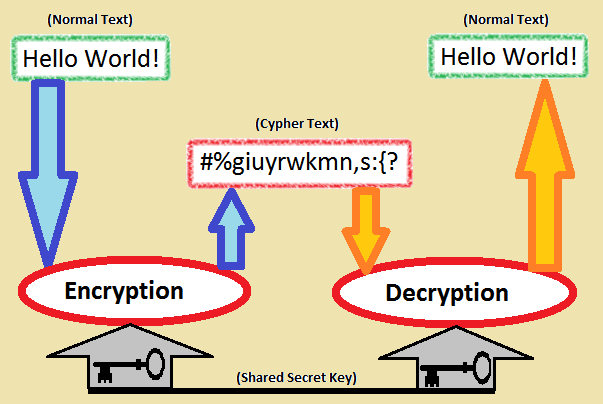
\includegraphics[scale=0.75]{pics/symmetric-key-crypto.eps}
\end{center}

\subsection{How does encryption work?}
Different approaches:
\begin{itemize}
	\item public key cryptography
	\item secret key cryptography
\end{itemize}

\subsection{How does encryption work?}
Different approaches:
\begin{itemize}
	\item public key cryptography (example: {\em RSA}, your ssh keys)
		\begin{itemize}
			\item Edward has a private and a public key
			\item data encrypted with her private key can only be decrypted by
				her public key and vice versa
			\item public key can be shared with Glenn
		\end{itemize}
\end{itemize}

\begin{center}
	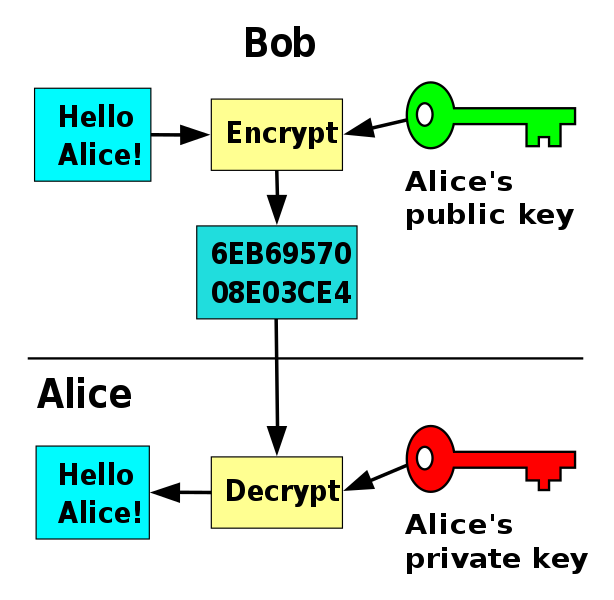
\includegraphics[scale=0.4]{pics/Public_key_encryption.eps}
 \end{center}

\subsection{How does encryption work?}
Different approaches:
\begin{itemize}
	\item secret key cryptography (example: {\em AES})
		\begin{itemize}
			\item Edward and Glenn share a secret key
			\item for authentication purposes, Edward may prove
				to Glenn that he knows the secret key
			\item any data encrypted with this key
				can also be decrypted using the same key
		\end{itemize}
\end{itemize}

 \begin{center}
        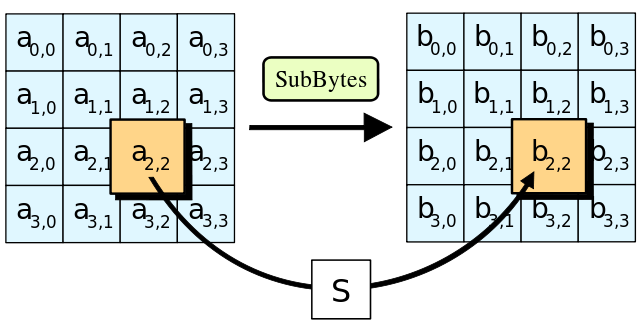
\includegraphics[scale=0.4]{pics/aes.eps}
 \end{center}

\subsection{Cipher Modes}
Encryption entails transformation of input data (``plain''
or ``clear'' text) into encrypted output data
(``ciphertext'').  Input data is generally transformed
in one of two ways:
\\

{\em Stream Cipher}: each bit on plaintext is combined
with a pseudo-random cipher digit stream (or {\em keystream})
\\

{\em Block Cipher}: fixed-length blocks of plaintext
are transformed into same-sized blocks of ciphertext;
may require padding


\subsection{Electronic Codebook Mode}
\begin{figure}[hb]
    \begin{center}
        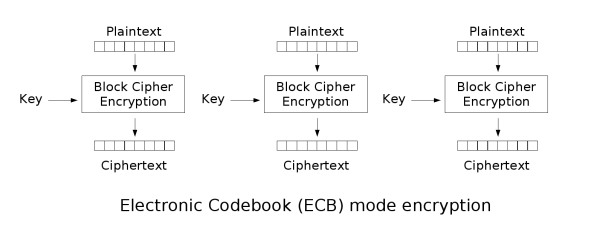
\includegraphics[scale=0.85]{pics/Ecb_encryption.eps} \\
        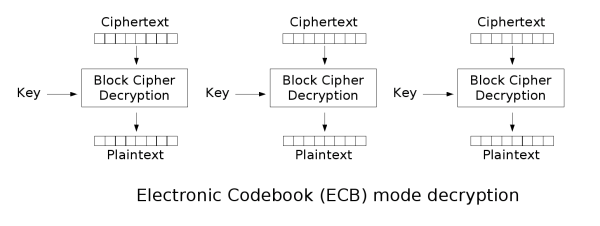
\includegraphics[scale=0.85]{pics/Ecb_decryption.eps} \\
    \end{center}
\end{figure}

\subsection{Electronic Codebook Mode}
\begin{center}
	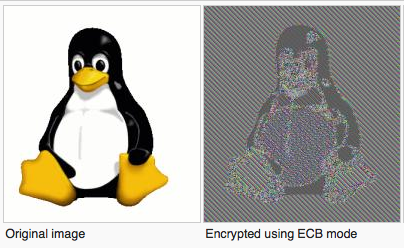
\includegraphics{pics/ecb.eps}
\end{center}


\subsection{Cipher Block Chaining}
\begin{figure}[hb]
    \begin{center}
        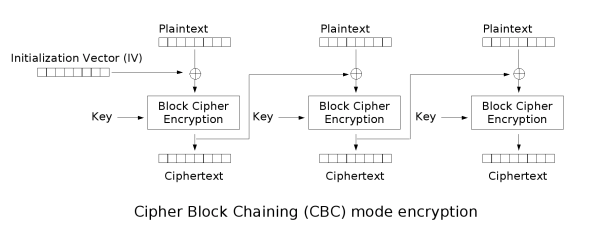
\includegraphics[scale=0.85]{pics/Cbc_encryption.eps} \\
        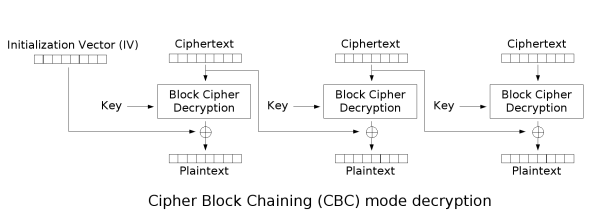
\includegraphics[scale=0.85]{pics/Cbc_decryption.eps}
    \end{center}
\end{figure}

\subsection{Random String generation}
Random numbers can be generated using {\tt /dev/random}, {\tt
/dev/urandom}, {\tt rand(3)}, {\tt random(3)}, {\tt BN\_rand(3)} etc.
\\

Map numbers to printable characters (for use as a salt, for example):

\begin{verbatim}
static const unsigned char itoa64[] =
        "./0123456789ABCDEFGHIJKLMNOPQRSTUVWXYZabcdefghijklmnopqrstuvwxyz";

char salt[16];
for (i=0; i<16; i++)
        salt[i] = itoa64[(int)random()%64];

\end{verbatim}


\subsection{Practical AES}
\begin{itemize}
	\item a symmetric block cipher
	\item variable key length
	\item consists of a key setup phase and the actual encryption or
		decryption
	\item keying material use of {\tt ivec}, which needs to be shared
	\item useful code examples in {\tt EVP\_EncryptInit(3)}
\end{itemize}


\subsection{HW\#4}
\begin{verbatim}
https://www.cs.stevens.edu/~jschauma/631/f15-hw4.html
\end{verbatim}
\begin{verbatim}

NAME
     aed - perform aes256‐cbc encryption/decryption

DETAILS
     aed reads data from stdin and either encrypts or decrypts it (depending
     on the -d or -e flag).  It uses AES 256bit CBC mode with a SHA1 digest
     with keying material derived from the passphrase using the
     EVP_BytesToKey(3) function, generating a suitable salt via RAND_bytes(3).

     Output is written to stdout.

     When encrypting, the output is prefixed by the string "Salted__",
     followed by the 8 byte salt.
\end{verbatim}
\Normalsize

\subsection{HW\#4}
\begin{verbatim}
https://www.cs.stevens.edu/~jschauma/631/f15-hw4.html
\end{verbatim}
\begin{verbatim}

     To encrypt the contents of the file ’file’ and storing the encrypted out-
     put in ’file.enc’:

           aed -e -p passfile <file >file.enc

     To decrypt the contents of that file again:

           aed -d -p passfile <file.enc

     Since aed operates on stdin and stdout, the above two commands could also
     be chained:

           export AED_PASS=$(cat passfile)
           cat file | aed -e | aed -d
\end{verbatim}
\Normalsize

\subsection{References}
\begin{itemize}
	\item {\tt crypto(3)}
	\item {\tt EVP\_EncryptInit(3)}
	\item {\tt EVP\_BytesToKey(3)}
	\item {\tt http://tldp.org/LDP/LG/issue87/vinayak.html}
	\item {\tt http://en.wikipedia.org/wiki/Cipher\_Block\_Chaining}
	\item {\tt http://www.moserware.com/2009/09/stick-figure-guide-to-advanced.html}
\end{itemize}

\end{document}
